\documentclass{beamer}

\usepackage[utf8]{inputenc}
\usepackage[T1]{fontenc}
\usepackage[english]{babel}
\usepackage{lmodern}
\usepackage{color}
\usepackage{fix-cm}
\usepackage{textpos}
\usepackage{eurosym}
\usepackage{multirow}
\usepackage{perpage}
\usepackage{eso-pic}

\graphicspath{{images/}}

\newcommand{\placetextbox}[3]{% \placetextbox{<horizontal pos>}{<vertical pos>}{<stuff>}
	\setbox0=\hbox{#3}% Put <stuff> in a box
	\AddToShipoutPictureFG*{% Add <stuff> to current page foreground
		\put(\LenToUnit{#1\paperwidth},\LenToUnit{#2\paperheight}){\vtop{{\null}\makebox[0pt][c]{#3}}}%
	}%
}%

% Redéfinis les marges des tableaux
\let\oldtabular=\tabular
\def\tabular{\small\oldtabular}
\renewcommand{\arraystretch}{1.5}

\usetheme{Warsaw}
\usecolortheme{orchid}

% Permet de réinitialiser les footnote à chaque frame. Nécéssite 2 compilations.
\MakePerPage{footnote}

\setlength{\TPHorizModule}{0.01\textwidth}
\setlength{\TPVertModule}{0.01\textheight}

\setbeamertemplate{navigation symbols}{}

\title{Dawwyd\\Reconnaissance Vocale}

\author[HOUDAYER \and RUHIER]{
	Benoit HOUDAYER\\
    \and
	Anthony RUHIER
}
\institute[SI75 - UTBM]{
    Gestion de Projet (SI75)\\Université de Technologie Belfort--Montbéliard}
\date{Février 2016}

\begin{document}

% Permet de masquer le comptage de slides
\bgroup
\makeatletter
\setbeamertemplate{headline}{}
\setbeamertemplate{footline}
{
  \leavevmode%
  \hbox{%
  \begin{beamercolorbox}[wd=.5\paperwidth,ht=2.25ex,dp=1ex,center]{title in head/foot}%
    \usebeamerfont{title in head/foot}\insertshorttitle
  \end{beamercolorbox}%
  \begin{beamercolorbox}[wd=.5\paperwidth,ht=2.25ex,dp=1ex,center]{date in head/foot}%
    \usebeamerfont{date in head/foot}\insertshortdate{}
%    \insertframenumber{} / \inserttotalframenumber\hspace*{2ex}
  \end{beamercolorbox}}%
}
\makeatother

\begin{frame}[noframenumbering]
 	\frametitle{}
	\titlepage
	\hfill
\includegraphics[height=1cm]{logo-utbm.eps}\hspace*{-1em}
\end{frame}
\egroup



% Ajout du compteur de slides
\expandafter\def\expandafter\insertshorttitle\expandafter{%
      \insertshorttitle\hfill%
      \insertframenumber\,/\,\inserttotalframenumber}

\begin{frame}
	\begin{small}
	\frametitle{Plan}
	\tableofcontents
	\end{small}
\end{frame}

\AtBeginSection[]
{
	\begin{small}
	\begin{frame}
		\frametitle{Plan}
		\tableofcontents[currentsection]
	\end{frame}
	\end{small}
}


%%%% Includes des sections :
%%%%%%%%%%%%%%%%%%%%%%%%%%%%%%
%
\section{le problème}
\begin{frame}
\frametitle{le problème}

Tâches secondaires :

\begin{itemize}
	\item écoute de musique
	\item consultation des actualités/météo
	\item réseaux sociaux
\end{itemize}

\end{frame}

\begin{frame}
	\frametitle{le problème}
	
	Tâches intrusives :
	
	\begin{itemize}
		\item écoute de musique $\rightarrow$ ouvrir le lecteur
		\item consultation des actualités/météo $\rightarrow$ ouvrir le navigateur
		\item réseaux sociaux $\rightarrow$ lire les messages des gens
	\end{itemize}
	
\end{frame}

\begin{frame}
	
	\frametitle{la solution}
	
	\begin{figure}
		\caption{L'utilisateur écoute de la musique en faisant la vaisselle}
		\begin{tabular}{cc}
		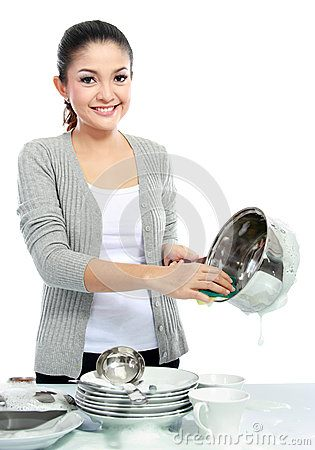
\includegraphics[height=6cm]{mains_mouillees} & 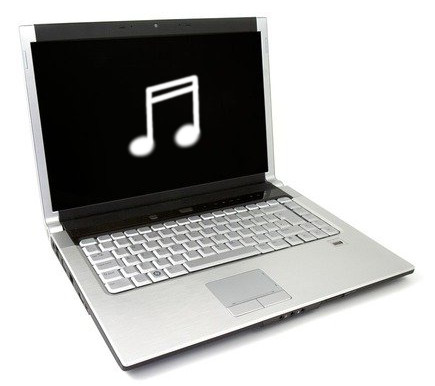
\includegraphics[height=3.2cm]{laptop_music}
		\end{tabular}
	\end{figure}
	
\end{frame}

\begin{frame}
	
	\frametitle{la solution}
	
	\begin{figure}
		\caption{L'utilisateur demande à Dawwyd de changer la musique}
		\placetextbox{0.46}{0.7}{"Dawwyd, musique suivante"}
		\placetextbox{0.59}{0.3}{\Large$\rightarrow$}
		\begin{tabular}{ccc}
			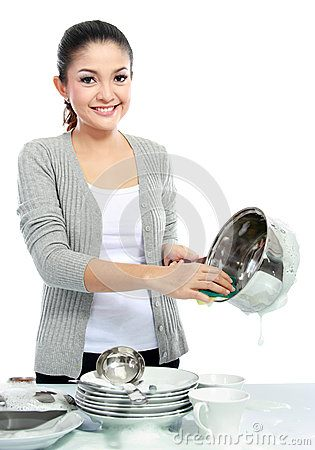
\includegraphics[height=6cm]{mains_mouillees} & 
\includegraphics[height=3.2cm]{hal_dawwyd} & 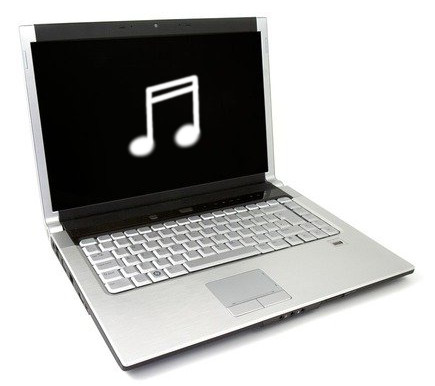
\includegraphics[height=3.2cm]{laptop_music}
		\end{tabular}
	\end{figure}
	
\end{frame}

\begin{frame}
	
	\frametitle{la solution}
	
	\begin{figure}
		\caption{Dawwyd a changé la musique}
		\begin{tabular}{ccc}
			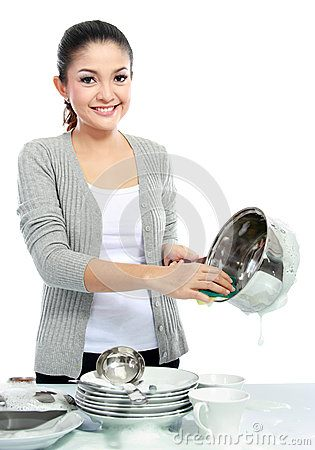
\includegraphics[height=6cm]{mains_mouillees} & & 
\includegraphics[height=3.2cm]{laptop_music_2}
		\end{tabular}
	\end{figure}
	
\end{frame}

\end{document}
